\chapter{Architecture}
\label{chap:architecture}

The following section will define the data model each peer keeps of its data and specify the API for updating it between peers, both trusted and encrypted.
Therefore we start this chapter with an explanation of all meta information that a trusted peer stores, as everything else is based on top of this information.
Then we will define and explain the model each peer keeps of the stored data.
Built on this model we will discuss the messages used to facilitate the update of the model between clients.
Then we will discuss the protocol extensions required for the encrypted model.
Finally we will take a look at the advanced features and how they can be built on top of the previous work.

We chose to use JSON for all communication between peers (see section~\ref{sub:JSON}).
Therefore generally speaking all messages will be defined as JSON messages.
Additionally most data is written to disk as JSON files.

\section{Meta Data}
\label{sec:Meta Data}

Since a trusted peer must store the last known state of the directory it is to synchronize to detect changes, we must store this information to disk somewhere.
For Tinzenite we took a page from Git and decided to write this information within the directory to be synchronized.
To reduce visual clutter and to hide it from users this directory is offered by a hidden directory directly below the root directory.
We specified it as \textit{".tinzenite"}.
In short it contains organizational files, temporary objects, and the deletion directory for storing files until they have been fully removed by all peers, plus data private to the peer.
Figure~\ref{list:meta_folder} gives a broad overview of the contents.

\begin{figure}[htp]
\begin{modellist}
\item .tinzenite/
\begin{modellist}
    \item org/
    \begin{modellist}
        \item peers/
        \item auth.json
    \end{modellist}
    \item removed/
    \item temp/
    \item receiving/
    \item sending/
    \item local/
    \begin{modellist}
        \item rmstore/
        \item model.json
        \item self.json
    \end{modellist}
    \item .tinignore
\end{modellist}
\end{modellist}
\caption[Meta Folder Structure]{Overview of the special meta information directory that Tinzenite uses to store relevant information required for the managing of the directory. For brevity sub directories that contain instance data are not expanded.}
\label{list:meta_folder}
\end{figure}

Placing the meta data within the directory has a few benefits for the complexity of the system and enables it to utilize the full feature set of the implemented synchronization capabilities to share data between peers when required.
Specifically only the \textit{"org"} directory and the \textit{"removed"} directory are synchronized as any user data, along with the \textit{".tinignore"} file which specifies to ignore all other objects.

\subsection{Organizational Directory}
\label{sub:Organizational Directory}

The \textit{"org"} directory consists of two objects: the file containing the authentication information and a sub folder which contains a file for each known peer.

\subsubsection{Authentication File}
\label{subs:Authentication File}

The authentication file stores information required for the complete Tinzenite network.
This includes information on the user, the directory the network synchronizes, and the encryption keys required to encrypt and decrypt data for encrypted peers.
Since the authentication file is not encrypted upon upload to encrypted peers as it is meant to be used to enable user account management, all personal or otherwise critical information is stored either hashed or fully encrypted.
Figure~\ref{json:auth_object} shows the contents of an example authentication file.

\begin{figure}[htp]
    \begin{lstlisting}[language=json,firstnumber=0]
    {
        "User": "$2a$10$E8Wlr9Jn/EYJLZ7J0yZoR.Qscp.MKD2kG8dHF7OQWYNA1mCfp.Qqe",
        "Dirname": "sync",
        "DirID": "ffff1d4cbfded232",
        "Secure": "Kbk4+sx17VKHma1Z67OU6R7TbHPWMr4SpZhWUQqheS/CNcKKHVYjTTSv0rbF4qDAa0vwikigsm7wHhy4iGjWB84i0ErO7rNwhqrPPxudeDM=",
        "Nonce": [255,142,165,173,201,188,98,116,29,31,173,181,84,84,137,54,159,50,193,248,51,162,76,195]
    }
    \end{lstlisting}
\caption[Authentication JSON Object]{An example of an authentication file.}
\label{json:auth_object}
\end{figure}

The key \textit{"User"} stores a bcrypt hash of the user's name~\cite{web:site:wiki:bcrypt}.
This is important for example for the support of encrypted third party peers: they can attach accounts to the provided user name for controlling server side access.
The user given name of the directory is stored in \textit{"Dirname"}.
We also need a way to distinguish multiple synchronized directories from each other: this is the random unique hash stored in \textit{"DirID"}.
Again, this can be used by third party service providers to differentiate the amount of directories that a user can store with them.
The encryption keys for encrypting and decrypting file data for encrypted peers is stored in \textit{"Secure"}.
These keys are encrypted with a password derived encryption scheme further discussed in section~\ref{sub:Encryption Scheme}.
\textit{"Nonce"} stores the nonce value that is required additionally to the user provided password to successfully access the encryption keys.

\subsubsection{Peer Files}
\label{subs:Peer Files}

Within the \textit{"peers"} folder Tinzenite writes all data synchronization peers.
It is in essence the contact list, filled with information required to access peers.
This includes a peer's address, trust, and further user defined information.

\begin{figure}[htp]
    \begin{lstlisting}[language=json,firstnumber=0]
    {
        "Name": "box",
        "Address": "b6ad2388839d3068f9d6562c10d1151dd87818373c88cf9aad829144c63aac36",
        "Protocol": 1,
        "Trusted": false,
        "Identification": "19baf5873da66797"
    }
    \end{lstlisting}
\caption[Peer JSON Object]{An example of a peer JSON object. Note that the encryption attribute is not to be trusted, it is only an optimization.}
\label{json:peer_object}
\end{figure}

Figure~\ref{json:peer_object} shows the structure of an example peer file.
One of these exist for all known peers.
The \textit{"Name"} is the user defined name for each peer, to be used by the user to make differentiating between peers easier.
Internally however the peer is referenced by the random assigned hash stored in \textit{"Identification"}.
The Tox address is stored in \textit{"Address"}.
Whenever a new peer is added and its peer file distributed to all known peers, they can use this information to automatically accept connections to the new peer.
The \textit{"Trusted"} attribute is an optimization: peers for which this value is false don't need to receive and decline a challenge.
It is important to note that the other way around is not true: if the value is false the other peer must still respond successfully to a challenge.
Finally the \textit{"Protocol"} value defines via which protocol the peer can be reached.
This is currently unused as we only use Tox.

\subsection{Removed Directory}
\label{sub:Removed Directory}

The \textit{"removed"} directory stores objects that are pending removal as described in section~\ref{subs:Remove}.
Each object is stored in a sub directory in this directory that is labeled according to their unique hash to avoid name conflicts.
Objects that are within this directory have a somewhat different model representation due to the need to acknowledge all removed objects throughout the network before being able to truly remove it permanently.

\subsection{Temporary Directory}
\label{sub:Temporary Directory}

The \textit{"temp"} directory is used for files that are peer local and is thus excluded from the synchronization by an entry in the \textit{.tinignore} file.
Objects for which this is the case is temporary models that the peer has received from another peer in the case that storing it is required.
More importantly Tinzenite uses this directory to store temporary files that are to be sent or received.
Receiving files are transmitted as blocks by Tox: therefore, to keep the RAM storage requirements down, these blocks are immediately written to disk within this directory.
This will also allow Tinzenite to resume downloads even in the case that the computer is restarted while the process is still in process (meaning even if the Tinzenite peer must restart).
Depending on the size of the file, files that are to be transmitted encrypted are also encrypted within this temporary directory.

\section{Peer Data Model}
\label{sec:Peer Data Model}

This section will describe our solution to how Tinzenite keeps track of objects within a directory.
This data will be henceforth referenced as the data model or just model.
The model is required to enable detection of newly created and removed files, since Tinzenite does not actively watch a directory.
Having a stored representation of a directory significantly eases the difficulty of detecting file creations and removals, even if the peer software is not running.
Any entry in the model is generally referred to as an object if the distinction between a directory or file is not required.

An important feature that the model should have is that it should represent an arbitrarily complex object structure in the most simple way possible.
Therefore there are only two assumptions we will make for the structure of any directory: namely that it contains files sorted in nested directories.
Out of this tree view we can immediately synthesize our two main components that we will require: a file model (a leaf) and a directory model (a node).
Since a peer is intended to have a directory as the root node from which to run, the core element will always be a directory.
An example of the proposed model structure can be seen in~\ref{list:model}.

\begin{figure}[htp]
\begin{modellist}
\item Root Directory
    \begin{modellist}
        \item .tinzenite Directory
            \begin{modellist}
                \item ...
            \end{modellist}
        \item Sub Directory
            \begin{modellist}
                \item File
                \item File
            \end{modellist}
        \item File
        \item File
    \end{modellist}
\end{modellist}
\caption[Data Model Example Structure]{An example of how a data model of a directory is structured. The .tinzenite directory is discussed in section~\ref{sec:Meta Data}.}
\label{list:model}
\end{figure}

Since each file is considered a binary blob and must not modified by Tinzenite in any way to preserve data integrity, any additional information that Tinzenite is required to store for an object must be kept within the model itself.
Out of this we can see which values need to be stored within the model for each object specifically.

Each object in the model will for identification purposes be specified by a unique randomly generated hash.
This hash allows us to decouple the name of the object from its model representation, effectively serving the same function as node identification numbers when stored on a disk.
Furthermore each model object will contain a path variable that specifies the relative path of the object in the directory tree.
This has the purpose of allowing the placement of all files in the correct locations on disk for a given root path.

\begin{figure}[htp]
    \begin{lstlisting}[language=json,firstnumber=0]
    "Version": {
        "927325d7a930dac9": 1,
        "19baf5873da66797": 4,
        "ec021135799691ae": 3
    }
    \end{lstlisting}
\caption[Version JSON]{An example of a version vector clock. Each hash is the identification of a trusted peer, the associated number which changes they last issued.}
\label{json:version_model}
\end{figure}

Apart from the above attributes Tinzenite must also track versions of files to allow detection of when objects have been updated.
We will use a vector clock~\cite{mattern1989virtual} to implement this, where entries represent peers and the associated number is the last version where that peer actively contributed to the object's history.
The vector clock can also be used to detect collisions.
Note that the vector clock must only store the versions for active, trusted peers as these are the only peers where versions can differ upon user interaction.
We avoid using a simple dirty flag for reasons of complexity: determining which peer's update to take in which order is not trivially doable with a simple boolean flag.
Utilizing vector clocks gives us greater flexibility, both for the implementation and for any visualizations in the case of tracing changes.
An example of the vector clock as we will use it can be seen in figure~\ref{json:version_model}.

It is important to note that the model will not be used to store peer reliant information.
This includes for example where the directory is placed on the peer's file system, which may differ between peers.
Such information must be stored separately by the peer and applied when working with the data model, for example when determining what the full path on the file system will be for a file that is to be written.
Some properties are also not suited to be transferred between peers.
This includes file system or operating system dependent properties such as usage rights, ownership, or flags.
For Tinzenite we will generally ignore these as primary focus is just raw data synchronization without semantic information.

\subsection{Directory Model}
\label{sec:dir_model}

\begin{figure}[htp]
    \begin{lstlisting}[language=json,firstnumber=0]
    {
        "Directory":true,
        "Identification":"db198086d1708794",
        "Name":"test",
        "Path":"test/test",
        "Shadow":false,
        "Version":{},
        "Objects":[]
    }
    \end{lstlisting}
\caption[Directory JSON Model]{An example of a directory JSON object. Note that for brevity no files or sub directories are shown in the \textit{"objects"} array. The version object is also left empty here.}
\label{json:directory_model}
\end{figure}

Figure~\ref{json:directory_model} shows an example of the proposed JSON structure for representing a directory.
A directory is somewhat special as it does not require the synchronization of an attached binary file.
This is the case for Tinzenite because directories are viewed independent from their content.

The \textit{"identification"} attribute is a random generated hash that uniquely identifies the directory.
The \textit{"path"} attribute stores the concatenated relative full path from the peers root directory to where the directory lies.
The clear text \textit{"name"} is also stored here as an attribute.
The \textit{"shadow"} flag is used to signal whether the contents of the directory are to be fetched or not.
To differentiate between updates we require a \textit{"version"} attribute which represents a vector clock of peers and their last known version.

Finally an \textit{"objects"} array is where the corresponding sub directories or files are recursively placed.
To model a directory as shown for example in figure~\ref{list:model} Tinzenite begins the model with directory model for the root directory.
Within the objects array are then the two files and the two further directories.
Each directory object in turn also stores sub objects in its object array, thus recursively modeling an entire directory.

\subsection{File Model}
\label{sec:file_model}

\begin{figure}[htp]
    \begin{lstlisting}[language=json,firstnumber=0]
    {
        "Directory":false,
        "Identification":"b83cf06d4e056e1a",
        "Name":"else.txt",
        "Path":"test/else.txt",
        "Shadow":false,
        "Version":
        {
            "927325d7a930dac9":1
        },
        "Content":"e4abda92f30700d751ac82f7454787d5"
    }
    \end{lstlisting}
\caption[File JSON Model]{An example of a file JSON object.}
\label{json:file_model}
\end{figure}

Figure~\ref{json:file_model} shows an example of the proposed JSON structure for representing a file object.
The \textit{"identification"} attribute is a random generated hash that uniquely identifies the file.
The \textit{"path"} attribute stores the concatenated relative full path from the peers root directory.
The clear text \textit{"name"} is also stored here as an attribute.
To differentiate between updates we require a \textit{"version"} attribute which represents a vector clock of peers and their last known version of this file.
Important for detecting file changes is the \textit{"content"} attribute which stores a hash of the file's binary blob.
Finally the \textit{"shadow"} flag is used to notify a peer whether the file is locally accessible or must first be fetched from other peers.

\section{Core Update API}
\label{sec:Core Update API}

This section describes the application interface that will be used to synchronize two models on separate peers where the models might diverge.
To understand how this works, it is important to understand how Tinzenite is structured.

Every peer views all connected peers as separate connections.
A swarm behavior only comes to pass because of the independent actions of every peer, not through a combined communication between multiple peers.
This primarily makes it relatively easy to implement a Tinzenite peer, as the communication state is never between multiple peers.
Therefore a single peer has a base state of no other connected peers.

\subsection{Connection Management}
\label{sec:conn_management}

In this section we will discuss how Tinzenite connects to other peers.
As we distinguish between trusted and encrypted peers we must determine how the data we will send is to be modified accordingly.
Note that encrypted peers by default will not initiate connections, only trusted peers as they are the only peers capable of working on the user's data.
Encrypted peers in general have a very passive role in the Tinzenite network.

Since each trusted peer has access to a list of all connected peers (see section~\ref{sub:Organizational Directory}) this list is used for the initial presumption what connected peer is trusted and which is encrypted.
Therefore peers marked as encrypted are not even issued the challenge.
To vet trusted peers however the challenge must be met.
Therefore the trusted peer queries each trusted connected peer in turn.
Since we should not trust a peer just because it has been marked as trusted, this query must be cryptographically secure.
An attacker that wants to connect to a trusted peer illegitimately thus can not establish a clear connection without the required keys, which they should not be in possession of\footnote{Tinzenite is designed to avoid revealing keys to outsiders. However attacks such as key loggers are beyond its control.}.
We define this as the authentication challenge.
Only if the challenge is successfully answered is the other peer considered trusted and the following communication not anonymous.
If the challenge is answered incorrectly or not at all we can not be assured that the other peer is either trusted nor encrypted, thus we simply ignore it for all further operations\footnote{Ideally we would warn the user of this as it may result in peers being orphaned within the network. As this requires either the user having tried to connect to an insecure peer or a peer having become corrupted, the chance that this behaviour is undesired is comparatively slim.}.
This concludes opening a communication channel with a connected peer.

\begin{figure}[htp]
\centering
    \includegraphics[width=6cm]{graph/sm_peer_communications}
\caption[Connection State Diagram]{This diagram shows how peers handle the establishment of a connection to a known peer.}
\label{graph:connection_states}
\end{figure}

Figure~\ref{graph:connection_states} shows an informal state diagram of how a peer reaches the idle state where the connection is ready and set up, both for trusted and encrypted peers.
The switch from the disconnected state to the connected state is signaled by the underlying Tox connection, meaning it happens when the other peer is online and visible via the Tox channel.
Once connected and if the peer itself is a trusted peer, a challenge is sent which contains an encrypted nonce.
For a more in depth look at the challenge response mechanism see section~\ref{}.

Note that a few points must be considered that can not be shown in the diagram.
Since Tinzenite is designed as a peer to peer network, no client server structure exists.
This poses the challenge of who begins the construction of a connection, especially as we can not distinguish between peers that have been online for a while already and peers that just activated when the base peer starts up.
This is due to peer to peer architecture of Tox: not all peers will respond to queries within the same time frame.
Peers further away from a network perspective will seem to be online only after peers that are nearer.
We solve this issue by having the peers use a random back off time whenever a request expects an answer\footnote{For example the challenge message for establishing a trusted connection.}.

Since we can not trust the other side of the Tox channel to be a Tinzenite peer, the peer initiating a connection will not advance beyond a step where it expects an answer.
This means that for example an attacker would either receive only a challenge (to which he can't respond without knowing the keys) or the request for the meta information block to which he'd have to correctly answer.

A short note on closing a connection: once established this happens when the underlying Tox channel is terminated.
Furthermore if something interrupts the establishment of a connection, both peers will simply reset to the starting point.
Establishing a connection is done every time a peer reconnects.

\subsection{New Connection Establishment}

The previous section described how Tinzenite connects to known peers.
This section therefore discusses how Tinzenite connects to new peers, meaning peers that the user adds to the network.
Notably this is a manual process where the user is used as a secondary channel to prevent man in the middle attacks.
Since a typical Tinzenite network might have many peers, it is not desirable to have to authenticate a new peer manually with every other peer.
We therefore propose that the user only need authenticate the new peer with one existing peer.
From there the authentication is synchronized to the other existing peers much like any other file or property update.
This bootstrapping process allows a user friendly setup of peers.
Should the same peer have been added multiple times at different existing peers Tinzenite will detect this and merge the authentication together.

\begin{figure}[htp]
\centering
    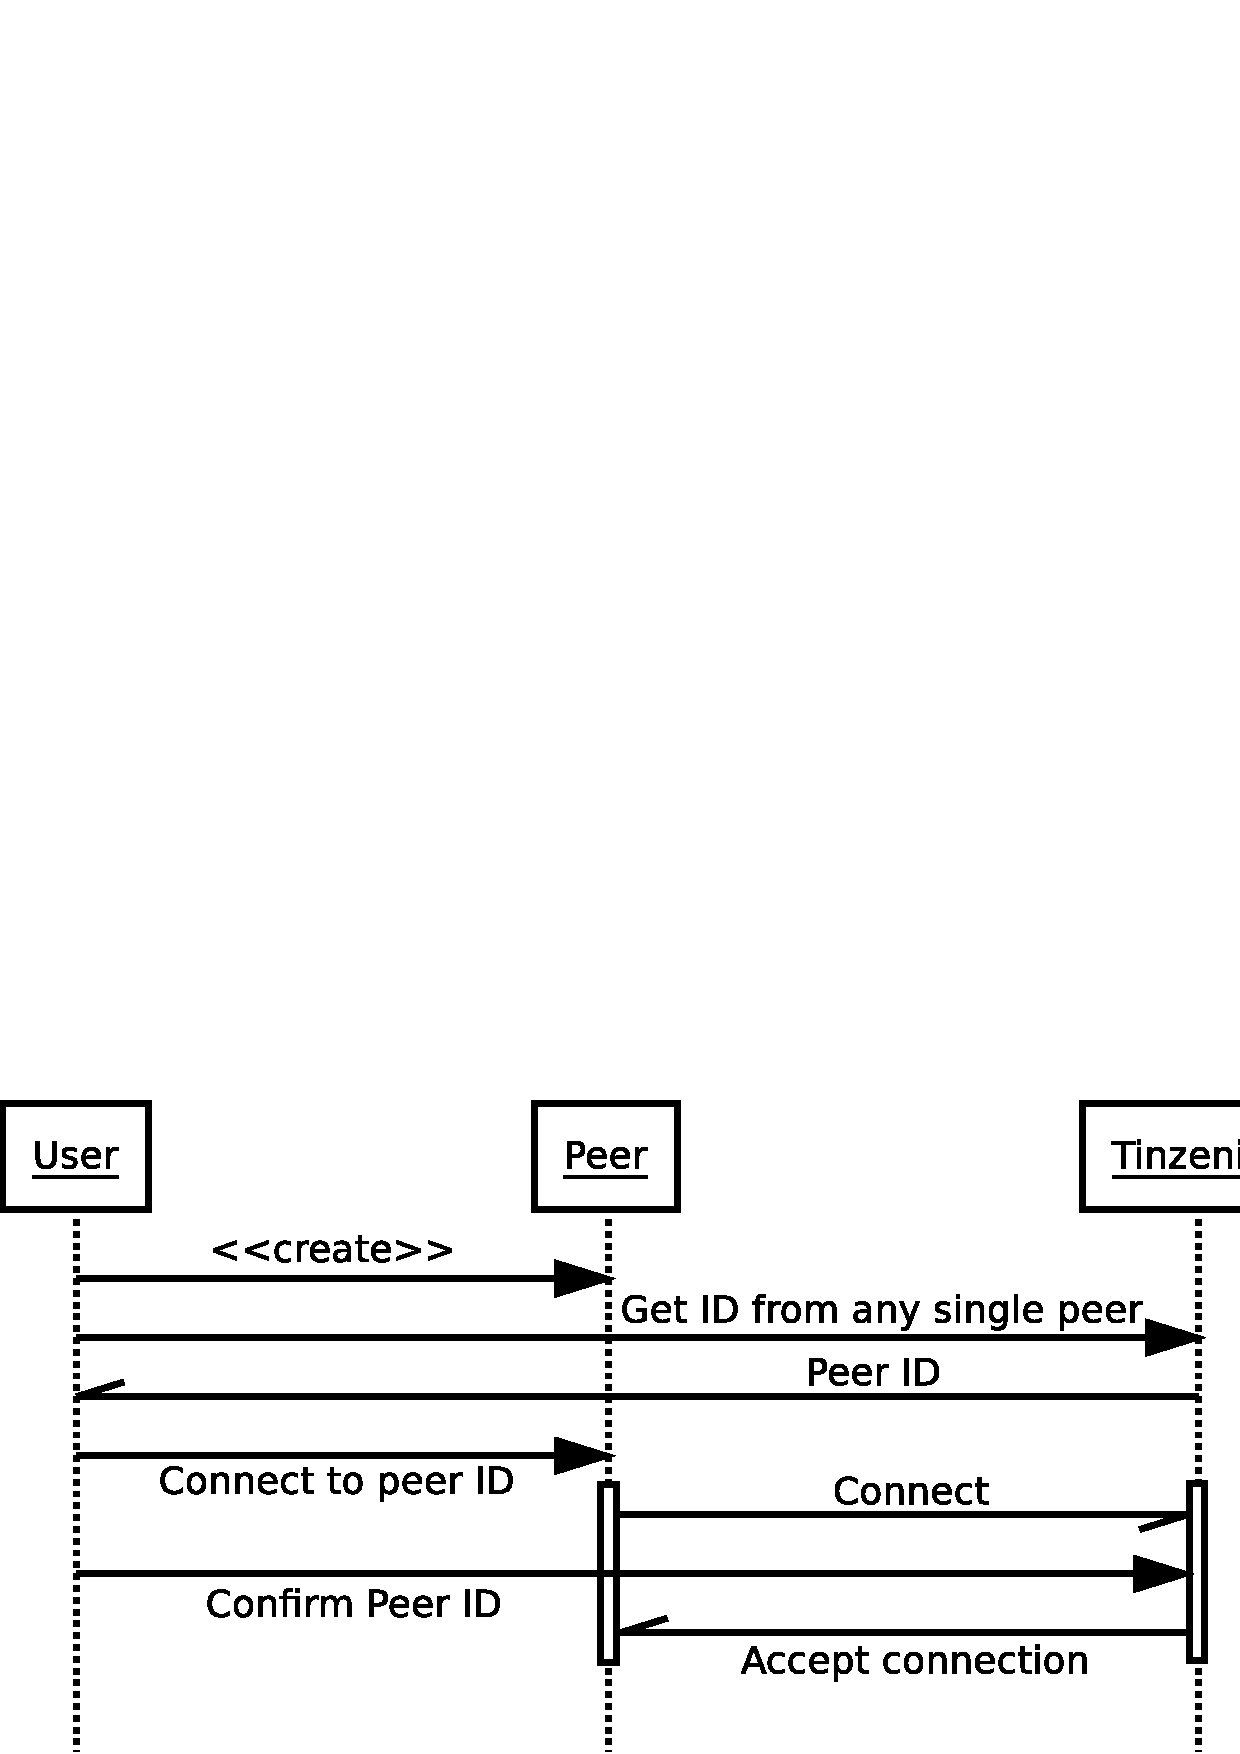
\includegraphics[width=10cm]{diagram/sequence_new_connect}
\caption[New Connection Sequence Diagram]{This diagram shows the interaction required to connect a new peer to the existing Tinzenite network.}
\label{diagram:new_connection}
\end{figure}

Figure~\ref{diagram:new_connection} shows how a user interacts with a Tinzenite peer and the Tinzenite network (consisting of 1 to n other existing peers) to connect a new peer to the network for the first time.
As prose: the users simply start the new peer client for the first time.
Then they can point it at the directory location, change settings, and check that another peer is visible.
To establish an initial connection a Tox ID of an available Tinzenite peer is required.
The users can then command the new peer to connect to this available peer by entering the Tox ID.
To ensure that no man in the middle attack can happen the users will now have to confirm the connection on the available peer.
This means allowing the connection there and ideally ensuring that the seen Tox ID is identical with the new peer's Tox ID.
Once the connection has been confirmed on the other peer a channel is opened.

The peer then receives the authentication block to set up the basic information it requires as part of the bootstrapping process.
Notably this also allows the user to define the new peer as a trusted peer by entering the password that unlocks the encryption key used for the stored data.
Access to the key also allows the peer to respond to other peers as a trusted peer.
The new peer address and its information will now be synchronized throughout the already connected peers once they are available, removing the need to add the new peer manually to each and every one.

Now the channel has been established and the peers can begin communicating as shown in figure~\ref{graph:connection_states}.
Notably though the starting state is the \textit{"Connected"} state as the connection has already been established on the Tox layer.
Depending on whether the user has specified the new peer as a trusted peer by entering the password or as an encrypted peer by skipping that step the peer will be defined accordingly.
The directories will begin synchronization once the challenge and model exchange have happened.

Removing peers will work much in the same way from a system perspective.
A user can note a peer to be removed, resulting in it being removed immediately from the peer where the action was initiated.
It will then transit through online peers and result in a complete removal once all peers have been online.
An interesting aspect to how to handle removal from the perspective of the to be removed peer is what to do with the data on the peer.
For a trusted peer we might offer a choice whether to remove the data or simply disconnect it from the Tinzenite network.
On the other hand encrypted peers can simply remove the data immediately as they can't access it anyway.

\subsection{Model Management}

This section will describe how a trusted peer receives and sends messages via the Tox channel.
Once the setup has been completed, as seen in section~\ref{sec:conn_management}, the models must be updated if they do not match.
This happens normally when files and directories have changed through user or system interaction.

\subsubsection{Request Operation}
\label{subs:Request Operation}

\begin{figure}[htp]
    \begin{lstlisting}[language=json,firstnumber=0]
    {
        "operation":"request",
        "request":"model|object",
        "object":"object_unique_hash",
        "delta":"true|false",
        "TODO":"ADD LIBRSYNC STUFF HERE"
    }
    \end{lstlisting}
\caption[Request Message]{Message used to request objects from another peer. Note that if requesting the model the object attribute can be omitted.}
\label{json:request_message}
\end{figure}

Figure~\ref{json:request_message} shows how a message to initiate a file transfer is structured.
Note that apart from the identification we require no further information – the model has been independently updated.
Now the peers need only actually get the binary files.
Upon receiving the message the other peer starts a Tox file transfer which the initiating peer knows to accept as it just requested it.

By switching the request attribute from object to model the other peer, whether encrypted or trusted, can be commanded to resend its current model.
In that case no further attributes are required and can be left out, although it may be possible to utilize the delta capability on large models.
This is required for example in the case that the other peer does not send singular object update messages for the reason of conserving power or bandwidth.
Thus periodically actively requesting a full model update will still allow updates to propagate independent of individual update messages at some point in time.

This message is also explicitly used to get an encrypted peer to initiate a file transfer of the requested file or the encrypted model.
The encrypted peer will most likely respond with a file transfer of the requested object if the trusted peer has successfully locked it.
If not, the trusted peer will receive lock denial messages until it has successfully locked the connection.

\subsubsection{Update Object Message}
\label{subs:Update Object Message}

\begin{figure}[htp]
    \begin{lstlisting}[language=json,firstnumber=0]
    {
        "operation":"create|remove|move|modify",
        "object":{
            ...
        }
    }
    \end{lstlisting}
\caption[Update Object Message]{The message broadcast by a peer to connected peers to notify that an update has happened. Operation can be any value of either create, remove, move, or modify.}
\label{json:update_object}
\end{figure}

Figure~\ref{json:update_object} is a message for broadcasting a model update to other connected peers.
The update message serves to keep both models in sync even after the initial synchronization at connection establishment.
Upon receiving an update message the peer will most likely immediately respond with a fetch message to retrieve the updated file.
If a peer receives a message for an operation that it has already applied, the message is silently discarded.
This does not disturb the propagation of updates since the peer will have already sent the update to the other connected peers if it has the update already.
In this way we ensure that every message propagates as far as possible without consuming unnecessary bandwidth\footnote{Peers are of course free to implement message sending in any way since the update messages are not critical for Tinzenite to work. Peers can simply only send update messages to a limited number of peers, down to none if bandwidth is scarce for example in the case of a mobile device.}.

\subsection{Encrypted Management}
\label{sub:Encrypted Management}

Communication with the encrypted peer is a special case as all operations on the encrypted files must happen on the trusted peer.
Since the encrypted peers can not resolve conflicts we must ensure that no conflicts ever happen specifically on the encrypted data.
We do this by ensuring that only ever one trusted peer may synchronize with an encrypted peer by utilizing a locking mechanism.

\subsubsection{Locking Operation}
\label{subs:Locking Operation}

\begin{figure}[htp]
    \begin{lstlisting}[language=json,firstnumber=0]
    {
        "operation":"lock",
        "lock":"request|accept|deny|remove",
        "nonce":"random_number"
    }
    \end{lstlisting}
\caption[Lock Peer Message]{Message for negotiating a lock for a peer.}
\label{json:lock_peer}
\end{figure}

Figure~\ref{json:lock_peer} shows the format of the message used to negotiate a lock for an encrypted peer.
The trusted peer first sends a request to which the encrypted peer can either answer with accept if no lock is currently active or deny if there is.
Once locked we must ensure that the encrypted peer will not become stuck in a locked state: we do this by having it implement a time out.
This time out resets after every received interaction from the trusted peer (so that we do not accidentally time out on long file transfers for example).
If the trusted peer tries an operation while locked out, the encrypted peer will respond with a denial message every time.
Once the trusted peer is done with its operations it should remove the lock by sending a remove message.
To make associating locks easier on both sides we include a random nonce for identification purposes within the message.

\subsubsection{Apply Operation}
\label{subs:Apply Operation}

\begin{figure}[htp]
    \begin{lstlisting}[language=json,firstnumber=0]
    {
        "operation":"apply",
        "subject":"model|object|remove",
        "object":"object_unique_hash"
    }
    \end{lstlisting}
\caption[Apply Message]{Message used to apply operations on an encrypted peer. Note that the object attribute isn't including if the subject is the model.}
\label{json:apply_message}
\end{figure}

Since files must also be uploaded to the encrypted peer we further require an apply operation message as seen in figure~\ref{json:apply_message}.
Notably the encrypted peer will overwrite any already existing encrypted object if the receiving object matches the unique identification.
This means the apply message can be used to both overwrite files with updates and create new files as needed.
To upload the new model to match the encrypted peer's files the subject is stated as model, resulting in the encrypted peer receiving a new encrypted model and replacing any old version with it.
To permanently delete files from the encrypted peer in the object removal case the subject is set to remove, with the object identification given.
On the topic of removing objects from encrypted peers and how it plays together with remvoing objects from trusted peers in a safe manner see also section~\ref{subs:Remove}.

\subsection{Message Timing}
\label{sub:Message Timing}

Now we must define when which messages are sent.
For the initial creation of a connection the order of messages can be seen in figure~\ref{diagram:new_connection}.
Once the connection is established we must differentiate between trusted peers and encrypted peers.

For trusted peers we propose the following message timing to enable rapid propagation of updates throughout the network.
Upon connection both peers will first exchange models, providing essentially a snapshot of differences since the last synchronization.
Peers will thus immediately begin updating each other so that the directory returns to the same state on both instances.
If local changes happen during or after the model has been exchanged the update messages are used to notify the other model of the update without having to retransmit the entire model again.
However to ensure that all updates do propagate at some point, ideally rather faster than longer, we propose that each peer resend the model every few units.
The exact spacing of when the complete model is resent is again up to the peer itself and can be adjusted per instance.
This allows mobile peers to work more energy efficient by synchronizing less often in comparison to desktop peers where power and bandwidth usage don't play a prominent role.

Since encrypted peers work passively it is again up to the trusted peers to ensure that they are queried regularly.
Once a lock has been established it is important that the trusted peer completes the exchange of models and files rapidly so that the encrypted peer can be unlocked again for other trusted peers.
This is enforced with a lock time out if no further messages are received from the trusted peer or it disconnects while locked.

From the user perspective we hope to offer easy to use and clearly labeled settings that allow great flexibility in how fast directory synchronization happens within Tinzenite for all relevant peers.
Therefore the client peer and the mobile peer will offer sane default values that can be modified if the user so wishes.
We will make sure to highlight the effects of setting the timing values to extremes of course as too great or too little time between messages will result in deficiencies for the user experience.

\section{Object Operations}
\label{sec:Object Operations}

In this section we will discuss the object operations that Tinzenite requires to work.
Then we will specify the actual architecture of the messages we require for them.
Finally we discuss how updates propagate through the network, especially concerning the differences between trusted and encrypted peers.

\subsection{Operations}
\label{sub:Operations}

Tinzenite relies only on the most basic file operations for manipulating both the model and the actual file directory.
Therefore we require only the following four operations for the basic case to work:

\begin{description}[leftmargin=5em,style=nextline,noitemsep,nolistsep]
    \item[Create]
        Files that have been created will be added to the model at the correct location and their attributes calculated, if not given.
        Tinzenite then checks whether it needs to fetch the file if it wasn't created in its own directory.
        Created files are detected by simply noticing files that do not exist in the model yet and are not listed as deleted.
    \item[Remove]
        File removing is one of the most complex cases in Tinzenite due to the insert delete ambiguity (see section~\ref{sub:Perspectives on Optimistically Replicated, Peer-to-Peer Filing}).
        We solve this by storing the models of deleted files until the delete update has propagated to all currently known peers.
        Only then is the model discarded also.
        For this to work Tinzenite must always ensure that files that exist but are listed as deleted are not added back to the model as a new file by continuously checking the deletion list.
    \item[Move]
        Moving a file could be represented as a remove followed by a create at the new location.
        For sake of complexity however we include a move command so that we can better represent both renaming operations and move operations.
        A move is detected if a file is removed and added somewhere else but retains its content hash.
        This allows detection of both move and renaming operations.
    \item[Modify]
        Modification is either when the model does not match the file anymore, in which case a new file must be fetched, or the content on the local file has changed.
        This is detected via the content hash.
        In that case the model is updated to match the file again.
\end{description}

These four operations are not the only operations that a user can do on directories or files.
However they are all the operations that Tinzenite requires so that it can offer full functionality.
Strictly speaking Tinzenite would actually only require three to work completely: the move operation can be replaced by remove and create (as discussed in section~\ref{sub:An Algebraic Approach to File Synchronization}).

\begin{figure}[htp]
\centering
    \includegraphics[width=4cm]{graph/sm_object_lifecycle}
\caption[Object State Diagram]{The life cycle of every object, file and directory, in Tinzenite with the allowed operations.}
\label{diagram:object_operations}
\end{figure}

Therefore the life cycle of an object is very simple, as can be seen in figure~\ref{diagram:object_operations}.
Objects can only come into existence via the create operation.
Objects can either be changed by changing their content, which is a modify operation, or by changing their location, which is a move operation.
Finally objects can also be removed.
If an object has been removed it will stay removed unless the user creates a new clone of it.

\subsection{Specifications}
\label{sub:Specifications}

In this section we show the actual definition of the specification and expand on how Tinzenite peers react to them in detail.
This specification makes up the core functionality of how the data synchronization happens within Tinzenite.
Note that these operations are only for trusted peers: since encrypted peers can not work on the stored data they have no need for the file operations.

\subsubsection{Create}
\label{subs:Create}

The creation of an object can be trivially detected in Tinzenite.
Basically there are two cases where an object must be created: the first is local manual creation which implies that the peer is the origin of the file; the second is creation via receiving an creation message from another peer.

For the first case, if the object does not have a representation within the model and is not listed as deleted, it triggers the creation case.
Tinzenite creates the correct object representation and inserts it into the correct place in the model.
In the second case the peer will queue a fetch operation for the required file\footnote{Note that in the case that it receives an update with a set \textit{"shadow"} flag it will not try fetching the file from said peer as it doesn't have a copy of the file. As a special case files within shadowed directories will also never be fetched.}.
Only when the file has been received completely is it placed at the correct location and the model updated.
Finally the update is propagated as specified in section~\ref{sub:Update Propagation}.

\subsubsection{Modify or Move}
\label{subs:Modify or Move}

The modification of an object is not as trivially detected as an object creation – for the specifics of update detection see the following section~\ref{sec:Update Detection and Reconciliation}.
Here we will only concern ourself with what happens once a modification has been detected.
Again we have two cases for triggering this case: a local file has been modified or the peer has received an update message.

If the modification is detected locally first we update the model to match and then initiate an update message.
The message is of the format as shown in figure~\ref{json:update_object} with the operation now reading \textit{"modify"} or \textit{"move"} instead accordingly.
If, on the other hand, we receive such a message, we queue the fetching of the updated file in the modify case.
Upon receiving the changes we apply them and finally propagate the update to the other connected trusted peers.
If the operation is a simpler move operation the change must not be fetched as it can be executed locally immediately.

\subsubsection{Remove}
\label{subs:Remove}

Finally the deletion of an object is the hardest case within Tinzenite because of the insert delete ambiguity as discussed in section~\ref{sub:Perspectives on Optimistically Replicated, Peer-to-Peer Filing}.
It is non trivial to ensure that an object deletion has been received by all required peers so that it truly and finally can be removed from the system.
A simple solution would be a list of all ever deleted objects, but unlike removed peers this list promises to grow quickly on often used synchronized directories.
Therefore we require a sort of garbage collection so that we can trim the list from deleted files that have been applied to all known peers.

For the base case we will look at how Tinzenite deletes an object that has been removed locally first, then discuss how the update propagates and what the other peers are required to do to ensure a safe and complete deletion.
If a deletion happens the object and object model are moved to a special directory outside of the user viewable directory (see also section~\ref{sec:Meta Data}).
Then the peer copies the list of currently known trusted peers\footnote{Note that encrypted peers must not be considered because they basically mirror only active peers, meaning they are guaranteed to correctly apply deletions once the active peers have reconciled it.} and places it with the object model.
Finally it creates a second list of peers in which it places itself.
This second list contains all the trusted peers that have acknowledged receiving the deletion update.

This deletion update is then propagated to the other peers.
Each peer receives the update, moves the object and updates the object model, enters itself into the second list, and propagates the update.
Once the last peer enters itself into the acknowledgement list, thus making it equal to the first list of peers, it propagates the update one final time and can then delete the object model from the deletion space and the actual object.
The completed deletion update then traverses the peers backwards, each in turn deleting the update from its list and propagating it a last time.
Thus when the last peer to receive the full deletion update removes the model, we can be assured that all relevant peers have removed the object.

It is not immediately obvious why this works even should new peers be created while the deletion update is in progress.
In fact this is only possible by adding a small modification to the outlined process.
To show that the solution can work with the small modification we need to look at the two cases that can happen for a newly created peer, differentiated by where it first connects to.
If it connects to a peer that has already received the deletion update the solution would work by default without any modification.
This is the case since the new peer would receive the object model where the object has already been deleted.
It must thus not be notified of the deletion.
If, however, it connects to a peer that has yet to receive the deletion update even though it has already happened, we have a problem.
The new peer is not listed among the peers that must acknowledge the update even though it has the object.
Without the modification, this could result in the file being reintroduced by the new peer, undoing the deletion in effect.

Therefore peers must expand the first list of known peers if a single criteria is met.
This criteria is relatively straightforward: when receiving a deletion update each peer first checks the list against its own known peer list and in the case that they differ add all missing entries to the deletion update.
If a newly created peer has connected it will already be within the list and thus be ensured to have the deletion update hang around until it has received it.

Now a final note on what happens should a peer receive a deletion update for an object that it doesn't know.
In this case the message can not simply be silently discarded as there is no other representation of the update in the object model.
This could lead to orphaned updates if the peer acts as a bridge between two peers that were previously directly connected.
Therefore unknown deletion updates should be propagated if possible.
However, since orphaned updates can only happen as long as the peer list has not been fully updated between all peers, this is a sufficiently unlikely case that we can live with it.
By adding a time stamp we can even detect orphaned deletion updates and warn the user to help in solving the issue.
Alternatively we can also warn if we have too many possibly orphaned updates, although this would signify a larger issue.

\subsection{Update Propagation}
\label{sub:Update Propagation}

There are two modes for propagating updates throughout the Tinzenite network.
The first case is when sending the updates to trusted peers; the other is updating encrypted peers.
For trusted peers the peer may send an update message.
Figure~\ref{json:update_object} shows how such a message might look.
At the latest the update propagates when peers exchange models as discussed in section~\ref{sub:Message Timing}.
It is then up to all receiving peers to update their models and fetch the file, then propagate the update recursively.

Encrypted peers serve only as storage space for trusted peers and it is thus up to the trusted peers to keep the encrypted peers updated to their own state, merging locally if required.
Encrypted peers are updated manually by the trusted peer and do not propagate update messages since they are passive communication partners\footnote{Actually encrypted peers are not allowed to send update messages as they can not be trusted to truthfully convey them. See section~\ref{sec:Security Considerations}.}.
Trusted peers thus update encrypted peers by updating them to match their own models.
If the model received from an encrypted peer has been updated by another trusted peer, it is up to the local peer to fetch all changes, apply them locally, update its model, then update the encrypted peer to match the merged state of all known changes.

\section{Update Detection and Reconciliation}
\label{sec:Update Detection and Reconciliation}

This section describes the theoretical side of the update detection: how we detect updates on file systems in a way that does not consume too much resources of the hosting computer.
Then we will discuss the interesting case of update reconciliation and how Tinzenite reacts to conflicts.

\subsection{Update Detection}
\label{sub:Update Detection}

Tinzenite continuously checks the directory against the model of the same (see also TODO).

TODO.
I'm not sure how I can implement this yet and whether I will use an external library for a file watcher.
I'll get back to this at a later point in time.

%TODO
TODO write.
Directories MUST always check sub directories for changes before you can delete or modify them (at creation time they are empty by default).
Can directories only be removed if all sub files are removed first?
This could be a sensible way to implement this...

\subsection{Update Reconciliation}
\label{sub:Update Reconciliation}

The core algorithm for how update reconciliation is done is another important element of Tinzenite.
The following section introduces it and discusses the ramifications for the system based on the initial model synchronization, leaving aside the per object update messages at first.
These will be discussed once the basic mode is understood.
Note that only trusted peers actively resolve updates, although reconciliation can happen for models received from both trusted and encrypted peers.

The reconciliation begins by receiving the model of the other peer.
The model is temporarily stored so that Tinzenite can work with it until the reconciliation has finished.
To guarantee that the directory remains consistent with the model right from the start we propose a simple rule: the model of the local directory is updated atomically with the successful reception of the binary object updates.

For each object in the received and temporarily stored model Tinzenite performs a series of checks.
For the sake of decreasing algorithm complexity we start with the easy case of file creation.
In this case the object has not previously been stored in the local model.
This is the case when a file has been newly created on a remote peer.
We can thus request the object from the remote peer without further logic required.

If the object is listed in the deleted list we can possibly ignore it outright.
This would mean that the other peer has not received the deletion message yet.
To avoid reintroducing already deleted objects they thus have to be ignored when reconciling.
If however the objected has been modified we must reconcile this conflict.

If the object has neither been deleted nor created it can only have been modified.
As this is where conflicts can regularly happen the case is somewhat more complex.
There are two simple paths here: if no modifications have happened either remotely or locally, nothing further must be done.
If changes have been made remotely but not locally we can simply request the updated object from the remote peer and are also done.
If, however, we detect both local changes that the remote peer does not know of and remote changes that are new to us we have found a conflict.

Tinzenite uses only the model objects to detect changes, specifically only the version attribute.
As shown in section~\ref{sec:Peer Data Model} the version attribute contains a list of peers and the last known version of the object they have.
From this list we only ever are interested in the versions of the remote peer and the local peer.
By comparing these two attributes between the versions that both peers have we can reliably detect how to proceed without losing data.

\begin{table}[htp]
\centering
\begin{tabulary}{\textwidth}{R || C | C }
      & Local object not modified & Local object modified \\
    \hline \hline
    Remote object not modified & Nothing & Nothing (It is up to the remote peer to actively fetch this update.) \\
    \hline
    Remote object modified & Fetch remote object and apply update & Resolve conflict \\
\end{tabulary}
\caption[Peer Object Version States]{This table shows the four possible cases that can result from comparing the versions between two peers.}
\label{table:version_states_possible}
\end{table}

Figure~\ref{table:version_states_possible} shows the four possible cases.
Since there is nothing to do independent of our local state if the remote peer has no modifications\footnote{This is the case because the other peer is responsible for requesting our local changes: the local peer has no obligation to actively push changes.}, Tinzenite will check this first.
This is done comparing the locally last known version of the object from the remote peer with the version the remote peer how has of the object from the temporarily stored model.
If it is equal we can continue on to the next object.

In the case that the remote object has a higher version number since the last synchronization we check first whether changes have been made to the local object.
If not we can simply request the new version of the object and apply it to our model.
However if we detect that our local object has also been updated we have ourselves a conflict.
How this conflict is resolved is discussed in the next section.

\subsubsection{Conflict Reconciliation}
\label{subs:Conflict Reconciliation}

As stated before Tinzenite considers files to be atomic entities and thus will not modify them itself.
Therefore no automatic conflict resolution will be implemented in the base Tinzenite system.
Thus Tinzenite must support the user in resolving conflicts.
We do this by clearly labeling conflicts by appending a special word to the object name, possibly also referencing which operation has happened (either create, modify, or remove).
So now we must store both versions of the conflict in a way that it can be easily resolved on any peer.

The solution we propose is in itself simple enough from a technical view.
Basically, we remove the old version of the object and replace it with the two conflicting versions.
As these are newly created files they can propagate through the network as any other object would, allowing the conflict resolution to happen even on peers that did not see the conflict initially.
It is then up to the user to either keep both versions (likely renaming them) or merge the changes into one object and removing the other.
Both cases will be propagated through the network as normal file operations.

So for an extreme example case consider the following: a file present on two peers is modified on one peer but deleted on another.
Now they synchronize and detect the conflict.
Since by definition the deletion can not already have fully propagated as the other peer still could modify the object the file is still present in the meta data directory (see section~\ref{sec:Meta Data}).
Therefore both peers can access the other's version of the object and reintroduce it in the user viewable directory as normal conflicting updates.
The deletion update will be overwritten by the higher version update of moving the file to its conflicting state, thus ensuring that it will not remain valid for long.

\section{Advanced Features}
\label{sec:Advanced Features}

In this section we will describe the features that we consider to be advanced features.
These will for the most part be implemented at a later stage and are not relevant for the core functionality of the Tinzenite system.

\subsection{Space Management}
\label{sub:Space Management}

One feature that should be implemented is that peers can have a limited amount of available space without breaking the protocol.
This feature can be used to control how much data a mobile device has to synchronize at any given time or for the server peer, thus allowing control over how large directories maximally are.

Each peer is required to enforce the size restriction given by itself.
If the size limit has been reached it should only allow further updates as shadow files.
The interesting case is of course what happens to files that are modified above the limit: we propose either making the file a shadow file as soon as it crosses the limit or allowing modifications to push the size above the limit.
Since shadow files are already part of the Tinzenite protocol no further protocol support for this feature must be considered.

\begin{figure}[htp]
    \begin{lstlisting}[language=json,firstnumber=0]
    {
        "operation":"info",
        "size_limit":"bytes_value",
        "size_current":"bytes_value",
        "message":"message_text"
    }
    \end{lstlisting}
\caption[Information Message]{Message used by encrypted peers to send the user messages.}
\label{json:info_message}
\end{figure}

For encrypted peers the enforcement of size restrictions must be handled by the active peers.
This in turn means however that encrypted peers must be capable of denying additional updates.
The message for this is defined as in figure~\ref{json:info_message}.
It is sent upon an apply message that exceeds the size limit after the file transfer is denied.
The trusted peer can then notify the user and possibly even immediately mark the file as a shadow file in the encrypted peers model.

\subsection{Ignored Objects}
\label{sub:Ignored Objects}

To allow a user to only synchronize objects that they consider important another advanced feature we would like to implement is the ability to specify files and directories to be ignored.
An example for how we propose to implement this feature is the Git source control management software~\cite{web:site:git}.
By specifying the paths to directories and files within a so called \textit{.gitignore} visibility of these can be finely controlled.

In Tinzenite we plan to implement this functionality in a similar manner.
The file containing these rules can be synchronized just as any other file at any level within a directory.
Any new objects detected by Tinzenite that are listed in this file will not be created within the model, effectively keeping it out of the system.
Since it may well happen that such a file is created at a later point and thus introduce an uncertainty in handling the to be ignored files we propose a simple solution: the file is only ever applied for object creations.
Once a file has been created within the model it will be modified and deleted as any other file within the system, independent on the ignore file.

This in turn however means that renaming or moving a file in Tinzenite will remove it from the model, deleting it everywhere.
Since we believe this to be a feature for more advanced users we will not make this feature a core aspect of the system.
Normal users should have little need for only synchronizing a selected subset of files.

\subsection{Shadow Files}
\label{sub:Shadow Files}

Depending on the location of a client a user may with to only access specific files without having to get an entire set or updates.
This is a nice feature to have in the case of space and bandwidth restricted devices such as mobile devices.
By selecting specific files the client will then only update or retrieve the corresponding files or directories, ignoring the rest.
This works by fully synchronizing the model and creating placeholder empty files for every shadowed file.
By selecting a shadowed file it can be unshaded, resulting in Tinzenite trying to fetch the binary blob normally with all updates until it is again shadowed.

Functionality for the shadow file feature is available via the shadow attribute.
It affects only files directly as the creation of directories is not significant from a size point of view.
The attribute only serves as a shortcut to set all files of a directory implicitly to being shadowed.
If files are marked as shadow files they are not updated on the disk, only their model.
By setting the shadow flag to true the client will then immediately try to fetch the binary file from connected and available peers.

Of interest are then a few edge cases.
First and most trivial: what happens to an already synchronized file when the shadow attribute is set?
We propose that the file is immediately removed although this could be expensive in terms of bandwidth if the users quickly change their mind again as the file must then be fetched all anew.
A more sophisticated approach would integrate the size restriction capability of the client as proposed in section~\ref{sub:Space Management}.
By setting the space limit to a number below the full size of the directory files will only be immediately removed if near the space limit.
If the user changes their mind the file may thus still be immediately available.

So what do peers do if they receive a model update where the shadow flag is set?
It is important to note here that the shadow flag is considered to be transient when synchronizing models, meaning its value is considered to be local only.
However it is still sent as it is used to determine for the receiving peer whether it can fetch an update if applicable from the other peer.
Again it is up to the peer what happens upon receiving a shadow file update: trivially a peer that has a non shadow copy of the file will ignore shadow updates as it can not fetch the binary file update successfully from it.
It will then have to wait for another peer to offer the update where the attribute is not set.

The better solution would be to introduce a third value for the shadow attribute: temp.
This value is to be set when the peer knows of an update and has applied it to its model but has not fetched the binary file update yet.
Note that this is a local value only and should not be sent to other peers: in that case all instances of temp should be removed with true.
When connecting to other peers the peer can then request all available files marked as temp and fully update them as required.
This approach has the added advantage of allowing a peer to notify the user that the file has been updated but not fetched yet.
We may also use this functionality to signal slow network transfer speeds: the user could at a glance see that the update is pending, possibly avoiding unnecessary conflicts.

The final edge case is an unpleasant one: what Tinzenite does not provide is a way to ensure that one full copy of the shadowed file is kept.
If the user marks a file as shadowed on all peers it may well happen that Tinzenite loses the file.
For now we propose to avoid this by explicitly warning the user of this possibility.
One way to mitigate this risk is by allowing user defined shadowed files only for specific clients: we can probably assume that any full desktop peer should always retain a full copy of the directory anyway.

%TODO: Is this a future work todo?

\subsection{Encrypted Peers}
\label{sub:Encrypted Peers}

The final advanced feature that is vital for the encrypted peer for third party support is how encryption is handled within the protocol.
Trigger for detecting that a peer is encrypted is when the challenge is not correctly responded or denied (if it outright fails Tinzenite probably should warn the user as it would mean that someone is trying to guess the response).
If the peer is already marked as a non trusted peer the challenge must never even be offered in the first case of course.
Once the other peer has been identified as an encrypted peer it is up to the local peer to enforce the correct encryption on files.

Explicitly this means that encrypted peers only receive encrypted blobs of files, not knowing what is in them and where to store them in relation to each other.
This is all right however: encrypted peers only store the list of all encrypted files with the encrypted directory model alongside.
Notable exception is the \textit{org} directory as previously discussed.
Encrypted peers must only be able to send and receive objects as requested by a trusted peer.
For this each binary encrypted file is stored with the name of its unique identification hash, allowing the encrypted peer to know which files to send and which to overwrite as required.

\subsection{File Versioning}
\label{sub:File Versioning}

Another advanced feature that would be very nice to have and close the gap of feature parity between Tinzenite and other existing services would be the capability to offer file versions built directly into the protocol.
Indeed the core protocol would not even have to be changed to support this: all that is required is the capability to keep old files for a specific time somewhere where the peer can reinstate them if the user wishes it.

Therefore all that is needed is a definition of space where these old files can be stored.
We propose placing these files in a further directory labeled \textit{"versions"} within the \textit{.tinzenite} directory.
For each file object a directory with the name of the file identification is created as required where old versions can be stored.
To differentiate the multiple copies each file must be uniquely named: we propose a simple number for each version that increments.

It is important to be able to limit the amount of versions stored to keep the size of the directory manageable.
We believe that this could simple be done by telling any single client how many different copies of files are to be stored, for example the last six.
If a new version is added and it exceeds this self imposed limit the peer can simply trigger a normal removal, thus deleting the version from all peers once the removal has propagated.

Further work could then be done to decrease the size of the versions by only keeping one base copy and storing only binary deltas.
Again this would require somewhat extensive work on peer logic but no change in the core protocol.
To differentiate full copies and delta files we propose an identifying name change would suffice: by appending a special marker behind the version number we could differentiate the type.
The actual synchronization of deltas or full binaries is again already fully implemented in the core protocol and would work as any other file.

\section{Security Considerations}
\label{sec:Security Considerations}

As stated in the motivation for this thesis (see section~\ref{sec:Motivation}) security and privacy are a primary concerns for this thesis.
As such we will give a brief overview of conceptual thoughts on the security of the proposed work.
Please note however that a full security review is not the goal of this work or within its scope.
Nonetheless we hope to offer something secure enough for practical usage.

First we will concern ourselves with a network of only trusted peers.
In this case Tinzenite should be very secure as long as the user ensures that no man in the middle attack happens on setting up initial connections between new peers.
All further communications are encrypted and authorized by Tox.
This in turn means that Tinzenite remains as secure as the software it is built on.
As with any software all security is for naught should the user make an error or allow the stored data to leak outside of Tinzenite.
This is especially true as Tinzenite does not offer protection from other programs reading out the stored data in a clear text directory as this would make intended changes increasingly difficult.

So what changes when the server peer or other similarly encrypted third party peers are given access to the network?
Not a lot for the communication: Tox still theoretically guarantees a fully encrypted and authorized data channel.
Since the to be stored data is encrypted on trusted peers before being sent, direct access to the user's data should also prove difficult, pending that the encryption algorithm is secure enough.

Since encrypted peers receive the model and all associated files only fully encrypted, this should not provide to be a problem from a security standpoint.
Trying to overwrite user data by replacing the binary blobs with random blobs is detected by trusted peers when comparing the unencrypted file with its hash from the unencrypted model: if they don't match the update can be marked as invalid and corresponding action taken.
Detecting a wrong model is trivially done by decrypting it and checking if it is valid syntax.

Some information is leaked however.
Since we encrypt on a per file basis it is theoretically possible to analyze file usage associated with size to identify pieces of the user's directory.
This is only made easier by the fact that file sizes are roughly the same whether encrypted or not, with an accuracy down to the block size of the encryption scheme.
The information leak could be mitigated by implementing the core protocol with encrypted oblivious storage~\cite{goldreich1987towards}: however this may well be worthy of its own thesis and thus not further considered here.

% TODO possible future work!

Possibly even more problematic is the clear text storage of the peer list even on encrypted peers as it can be used to determine the size of the user's Tinzenite peer network.
However to allow encrypted peers to facilitate file transfer between two mutually exclusively online peers, it must know this information.
This is mitigated by the fact that Tox IDs are hard to guess and not shared beyond the Tinzenite peer network.
They however can be used to monitor the user's devices by utilizing the Tox distributed hash table to get current internet protocol addresses\footnote{TODO: IIRC Tox actually mitigates this via a form of onion routing. Take a look if the sentence is correct!}.

A further note on the challenge response part when establishing a known connection between two peers, as seen in section~\ref{sec:conn_management}.
We have defined that the connection is not established if the response is invalid.
As a bonus feature a client may well even actively warn the user of the invalid response, allowing the user to decide how to react correctly.
The user could either remove the peer from the directory network or initiate it anew so that everything returns to working order.
It should never happen that an encrypted peer answers invalidly even once if the system is not compromised and running as specified.
Therefore we may consider immediately removing the peer as if the user had manually removed it to ensure tighter security – of course the fact that a peer had been removed should still be immediately communicated to the user.

TODO: change the auth.json file to include trusted peer list.
Thus even peers can be sent only encrypted save for the list in auth.json which is used to determine if a peer may connect by the encrypted peer.
It is then important the clear version of the auth.json file is NEVER pulled so that no peers can be introduced by the server peer.

\subsection{Encryption Scheme}
\label{sub:Encryption Scheme}

TODO: explain how we encrypt files for encrypted peers, where and how the keys for that are stored, and expand on the algorithm to encrypt the stored keys with PRNG.
